\chapter{Firm-growth statistics}
\label{chap:firmgrowth}

\section{Firm-growth statistics in the fluctuating state}
\label{sec:growing-observables}

We measure the two firm-growth facts on the relative sizes $S_i = x_i/m$ of
Section~\ref{sec:growth-churn}, whose
cross-sectional mean is one by construction. The common growth of the economy is divided
out in the same step, since $\ln S_i = \ln x_i - \ln m$, so the size and its
growth $g_i = \Delta \ln S_i$ are the idiosyncratic part of a firm's trajectory, exactly
what the data measure. As in the empirical protocol, each firm contributes while it
is listed, that is while $S_i$ stays above the immigration floor, and we read growth
rates over a fixed yearly horizon $\Delta t$. All
statistics are taken in a late window, after the initial relaxation has passed, and
restricted to firms that persist across it. They are also taken at $N \ge 8000$: at
smaller sizes the fluctuating state is fragile, and at $N = 2000$ nearly half the graph
realizations collapse onto a fixed point and freeze, while from $N = 8000$ upward every
realization in our ensembles persists.

Two cautions, detailed in Appendix~\ref{app:numerics}, shape the measurement. The
per-firm volatility is a mean-absolute-deviation estimator robust to the fat tails, and
the size--volatility relation is fitted only over its power-law range, the decline above
the small-firm plateau set by the immigration floor. The same appendix varies the
horizon $\Delta t$ and the solver tolerance. The moment ratios are insensitive to both;
$\beta$ is stable for horizons up to the correlation time and drifts upward beyond it,
and the kurtosis falls with the horizon throughout, so the values quoted below refer to
the yearly horizon, as the empirical ones do.

Figure~\ref{fig:growing-msb} shows both observables at the operating point
$\mu = -1.76$, $\sigma = 1.75$ marked in Figure~\ref{fig:phase-diagram}, in the
stationary fluctuating state, for twenty independent economies of $N = 16000$ firms
each. The size--volatility relation (left) falls
monotonically over the fitted range, $\sigma(\bar S) \sim \bar S^{-\beta}$ with a
per-economy exponent
$\beta = 0.45 \pm 0.06$ across realizations. Large firms are less volatile than small ones, as in the
data. The growth-rate distribution (right) is
sharply peaked and fat-tailed, with both flanks heavier than the Laplace reference and
no systematic asymmetry between them (Bowley skewness $+0.01$).

\begin{figure}[htbp]
    \centering
    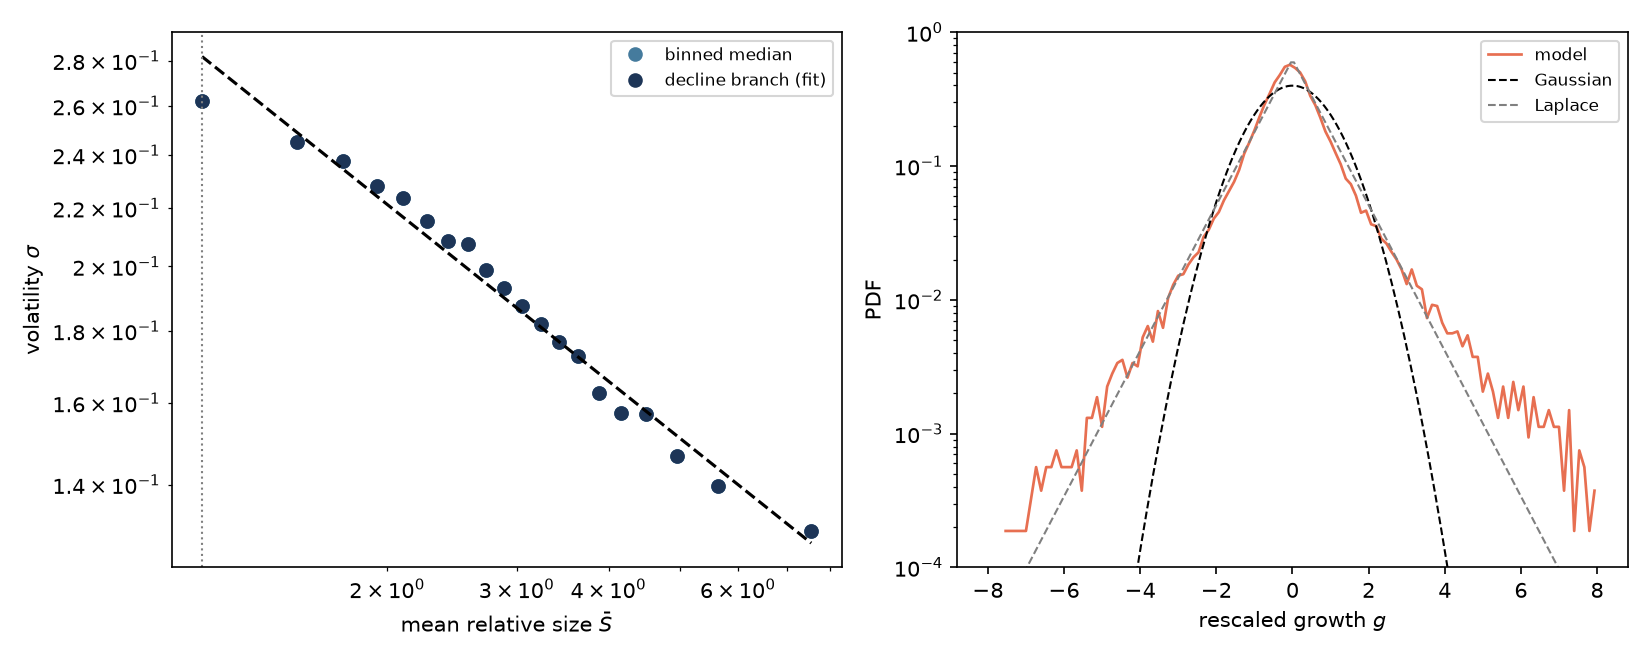
\includegraphics[width=\linewidth]{meandeg_stationary_msb.png}
    \caption{Firm-growth statistics at $\mu = -1.76$, $\sigma = 1.75$, pooled over twenty
    economies of $N = 16000$ firms on the power-law graph
    ($C = 400$, the fixed dilution $C = N/40$). \panel{Left}: the
    size--volatility relation; volatility falls as a
    power law over the fitted decline above the small-firm immigration-floor plateau,
    with per-economy exponent $\beta = 0.45 \pm 0.06$ and $R^2 = 0.99$. \panel{Right}: the
    growth-rate distribution, sharply peaked and fat-tailed,
    heavier than the Laplace reference on both flanks and close to symmetric
    (Bowley $\approx 0$), far above the Gaussian.}
    \label{fig:growing-msb}
\end{figure}

\section{Measuring exponents across realizations}
\label{sec:growing-estimator}

Every exponent in this chapter is measured over many graph realizations, and how the
realizations are combined affects the result. Each economy carries its own
overall volatility scale, set by its particular draw of the couplings, and these scales
differ by large factors from one realization to the next. The obvious estimator pools
the firms of all economies into one sample and fits the size-conditioned moments once.
But conditioning on size across pooled economies then compares a quiet economy's large
firms with a loud economy's small ones, which injects size-independent variance into
every conditional moment. The injected variance flattens the fitted slopes, more
strongly the higher the moment, so the pooled estimator biases every $\zeta_q$ downward,
bends the ratio curve $\zeta_q/\zeta_1$, and the bias does not shrink as more
realizations are added: pooling more economies is not more data for this purpose but
more mixing.

We therefore use the quenched estimator throughout: each exponent is fitted inside a
single economy, on that economy's own decline branch, and the exponents are then
averaged over realizations, with the quoted uncertainty the standard error of that
average. The two estimators disagree materially. At the operating point of
Figure~\ref{fig:growing-msb} the pooled ratios come out $1,\,1.77,\,2.32,\,2.67$ while
the quenched ratios are $1,\,1.84,\,2.51,\,3.02$, a disagreement large enough to
reverse a verdict.
All claims below are therefore quenched, and the pooled values are
reported only for comparison.

\section{Higher moments and the multiscaling}
\label{sec:growing-multiscaling}

The size--variance exponent is only the first moment of a richer object, the distribution
of growth volatility conditional on size, and it is on the higher moments that the
granular models break. \citet{moran2024} measure the $q$-th moment of the
size-conditioned volatility, $E[\sigma^q \mid S] \sim S^{-\zeta_q}$, and find an exponent
that depends on the order $q$: in the data
$\zeta_1,\dots,\zeta_4 \approx 0.20,\,0.39,\,0.51,\,0.58$. Their granular models predict
instead that the three higher moments ``decay with size all with the same scaling'', a
$q$-independent exponent, and it is this prediction the data contradict. As the
introduction set out, two reference lines bound the observable. The granular tail flattens
the ratio curve $\zeta_q/\zeta_1$ to a constant beyond $q=1$; a conditional volatility
with a single scale (a fixed distributional shape whose level alone slides with size)
locks the exponents to the first, $\zeta_q = q\,\zeta_1$, a straight line. The data lie
between them, rising with $q$ but sublinearly, and it is this $q$-dependence, which we
call the multiscaling of the size-conditioned volatility, that a model of firm growth must
reproduce. (\citet{moran2024} read the shortfall below the straight line as a subleading
correction from the incipient tail of their volatility distribution; whether the empirical
sublinearity survives asymptotically is open, and our comparisons are made at the moments
and sizes that are measured.)

Figure~\ref{fig:growing-multiscaling} makes the same measurement in the model, the
first four moments of the size-conditioned volatility, with each economy fitted on
its own decline branch. The quenched exponents rise with the order,
$\zeta_1,\dots,\zeta_4 = 0.41,\,0.76,\,1.03,\,1.24$, with standard errors
$0.01,\,0.03,\,0.04,\,0.05$ over twenty economies; the first is the size--variance
exponent of the previous section. Divided by $\zeta_1$, the
$q$-dependence is $1,\,1.84,\,2.51,\,3.02$ (each $\pm 0.01$--$0.04$), which lies on the
empirical $1,\,2.0,\,2.6,\,2.9$ through $q = 3$ and slightly above it at $q = 4$, and is
separated from the fixed-shape line $\zeta_q/\zeta_1 = q$ by many standard errors at
every $q \ge 2$ (right panel). The ratio curve is converged in system size,
$\zeta_4/\zeta_1 = 3.09,\,3.02,\,3.06$ at $N = 8000$, $16000$, $32000$, and
Appendix~\ref{app:scaling} carries the finite-size study across all topologies. Two
differences in shape remain: the
empirical curve saturates hard after $q = 3$ while the model's bends more gently, so the
model matches the data's values but not its curvature at the highest moment measured;
and the empirical exponents themselves are about half the model's, the magnitude gap
studied in Appendix~\ref{app:scaling}.

\begin{figure}[htbp]
    \centering
    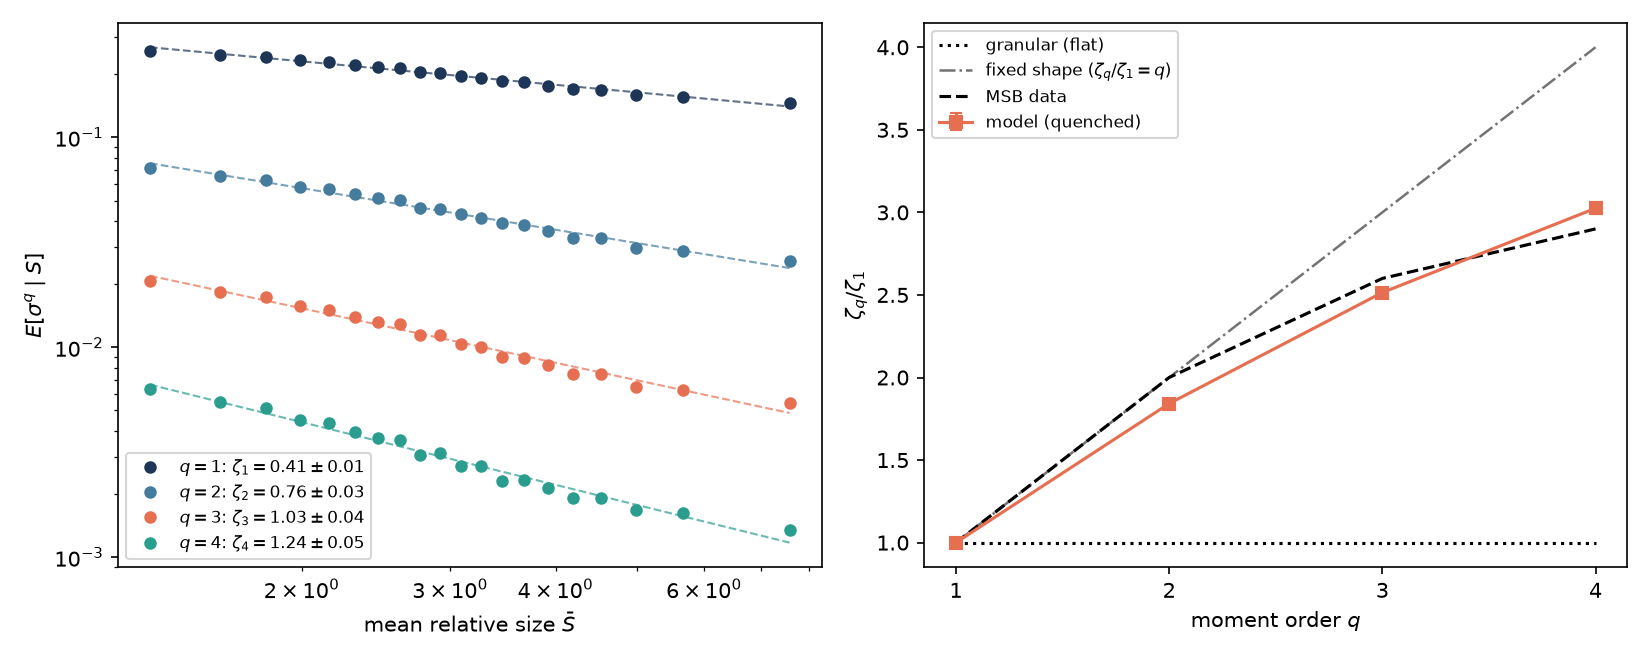
\includegraphics[width=\linewidth]{meandeg_multiscaling.png}
    \caption{Multiscaling of the size-conditioned volatility,
    $\mu = -1.76$, $\sigma = 1.75$, twenty economies of $N = 16000$.
    \panel{Left}: the first four moments $E[\sigma^q \mid S]$
    against mean size on a double-logarithmic scale, each fitted on the decline branch;
    the slopes steepen with the order $q$, the quenched exponents
    $\zeta_1,\dots,\zeta_4 = 0.41,\,0.76,\,1.03,\,1.24$. \panel{Right}: the exponents
    normalized by the first, $\zeta_q/\zeta_1$, against the moment order, for the model,
    the data of \citet{moran2024}, the granular prediction of a $q$-independent
    exponent, and the fixed-shape line $\zeta_q/\zeta_1 = q$ of a conditional volatility
    with a single scale. The model bends below the fixed-shape line onto the empirical
    curve: the shape of the volatility distribution broadens with firm size.}
    \label{fig:growing-multiscaling}
\end{figure}

The multiscaling is the first of three size-conditioned tests by which \citet{moran2024}
separate the data from the granular models, and the model passes the
other two as well (Fig.~\ref{fig:growing-conditional}).

The second asks how the spread of firm volatilities depends on size. Divide each firm's
volatility by the mean volatility at its size, $\sigma_i/\bar\sigma(S)$, and the resulting
distribution should be the same at every size, with a bounded tail. The model reproduces this
collapse onto a single size-independent shape, with a thin tail (the $99$th percentile
sits at $2.2$ times the median when the rescaling is done per economy), and the collapse
tightens, rather than degrading, as the system grows. The granular models predict a
second feature here: large firms built from only a few sub-units keep a fixed volatility that
does not shrink with size, which would show up as a hump in the rescaled distribution.
\citet{moran2024} find no such hump in the data, and the model shows none either; it has no
sub-units to produce one.

The third test turns on the central limit theorem. If a firm
were an aggregate of many independent parts, its growth would look more Gaussian the larger
it grew, so the excess kurtosis of its growth would fall toward zero with size. In the data
the excess kurtosis does not fall with size;
large firms stay at least as fat-tailed as small ones. The model reproduces this: the
excess kurtosis of the size-unmixed growth $(g - \bar g)/\sigma_i$ rises from about two for
the smallest firms to about six for the largest, a trend of $+6.5 \pm 0.5$ per decade of
size measured economy by economy, positive in every one of the twenty realizations. A
firm's growth here is not a
sum of independent contributions, so no central-limit averaging thins its tails as it
grows.

The model thus clears not only the size--variance exponent that the granular models also
fit, but every conditional test by which the data reject them.

\begin{figure}[htbp]
    \centering
    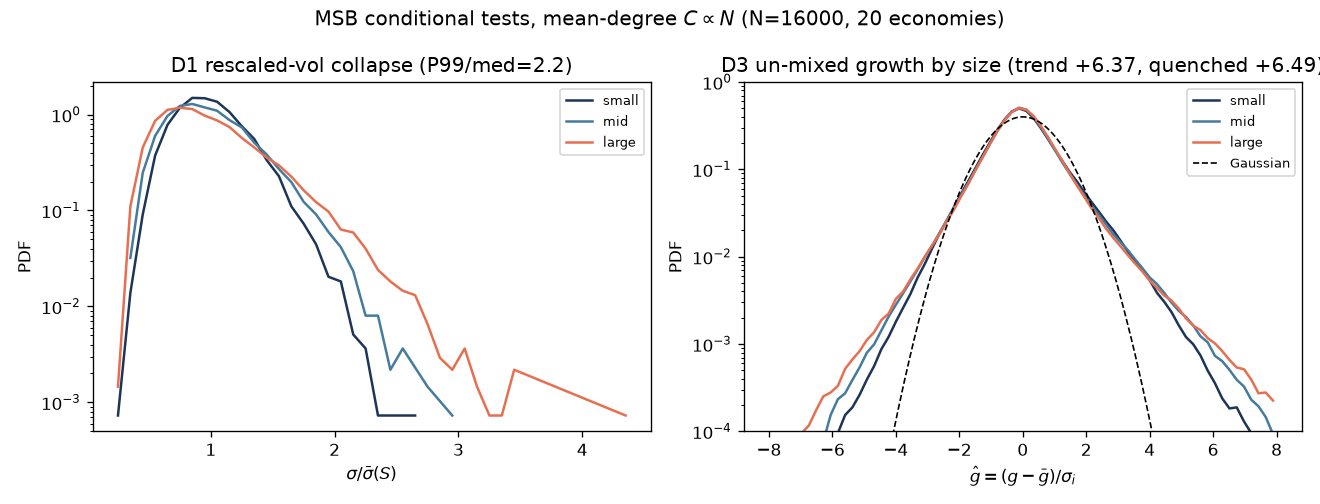
\includegraphics[width=\linewidth]{meandeg_conditional.png}
    \caption{The other two discriminating tests of \citet{moran2024}, twenty economies of
    $N = 16000$. \panel{Left} (second test): the per-firm volatility distribution, rescaled by its
    size-conditional mean $\sigma_i/\bar\sigma(S)$, collapses onto a single size-independent
    shape with a bounded tail. \panel{Right} (third test): the size-unmixed growth $(g-\bar g)/\sigma_i$
    stays fat-tailed at every size, well above the Gaussian, and the larger firms are
    fatter, the excess kurtosis rising with size in every realization; an aggregate of
    independent parts would approach a Gaussian.}
    \label{fig:growing-conditional}
\end{figure}

\section{The role of the graph}
\label{sec:growing-graph}

The couplings put two ingredients into the model, the quenched disorder on the
edges and the heterogeneous degrees of the graph that carries them, and the two can be
separated. Under the standard normalization \eqref{eq:coupling-global} every edge is
divided by the same mean degree, so the variance of the disorder field a firm feels
grows with its own degree, $\mathrm{Var}\,h_i \propto k_i/C$, the same degree-dependent
field that the heterogeneous mean-field theory of \citet{aguirrelopez} carries as a factor
$\sqrt{k_i/C}$ on its noise, so a firm's degree sets the level of noise it feels. If the
multiscaling is really the shape of the volatility distribution broadening with size,
this can produce it, and removing the degree heterogeneity should
then remove the multiscaling as well.

Figure~\ref{fig:growing-topology} repeats the full measurement with only the degree
distribution swapped; the disorder, the operating point and the mean degree $C = N/40$
stay fixed. On the homogeneous graphs the
multiscaling vanishes exactly: the fully-connected control gives ratios
$1,\,2.00,\,3.01,\,4.00$ and the regular graph $1,\,1.99,\,2.95,\,3.87$, the
fixed-shape line to within error. As the degree distribution broadens the ratio curve
bends away from that line, and only the power-law graph with infinite degree variance
(exponent $2.5$, the graph of every other figure in this chapter) reaches the empirical
curve. The size--variance exponent moves with the same parameter, from $\beta \approx 1$ on
the homogeneous graphs down through $0.73$ (power-law $3.5$) and $0.43$ (power-law $2.5$)
to $0.17$ (power-law $2.2$), inside the empirical band at this size:
degree heterogeneity is what pushes the exponent down toward, and through, the empirical
range. The tail exponent of the graph is thus a single control parameter that carries both
size-conditioned observables across the empirical values: the data are bracketed
between exponent $2.2$, where $\beta$ is right and the ratios run slightly low, and
$2.5$, where the ratios are right and $\beta$ is high. Pushing the tail harder still
(exponent $2.1$ and below) overshoots: $\beta$ falls below the band while half the
realizations freeze and the ratio measurement degrades, so the empirical pair sits at
the heterogeneous but still stable edge of the family. The
growth tent, by contrast, is indifferent to all of it, fat and symmetric on every
topology including the fully-connected one, so the tent belongs to the disorder alone
while the size-conditioned structure belongs to the graph.

The power-law-$2.2$ graph, the bracketing partner that carries the empirical exponent,
passes the full battery of conditional tests as well. Run at the same operating point
and size as the headline measurements ($N = 16000$, twenty economies, all surviving),
it gives $\beta = 0.21 \pm 0.07$, inside the empirical band at a size where
Appendix~\ref{app:scaling} shows this exponent converged; quenched ratios
$1,\,1.79,\,2.36,\,2.72$, tracking the empirical curve from below; a
rescaled-volatility collapse as tight as the headline graph's (tail $P_{99}$/median
$2.0$ against $2.0$ at exponent $2.5$, with size-independent medians); a size-unmixed
kurtosis rising with size at $+5.8 \pm 0.6$ per decade, positive in nineteen of the
twenty economies; and a symmetric fat tent (Bowley $+0.02$, excess kurtosis $10.5$).
The two bracketing exponents therefore fail in different places and by very different
margins: at $2.2$ the worst deviation is the highest ratios running $5$--$7\%$ below
the data, while at $2.5$ the ratios sit on the data but the exponent overshoots the
empirical band by a factor of two and is still drifting. Every conditional test is
passed at both.

\begin{figure}[htbp]
    \centering
    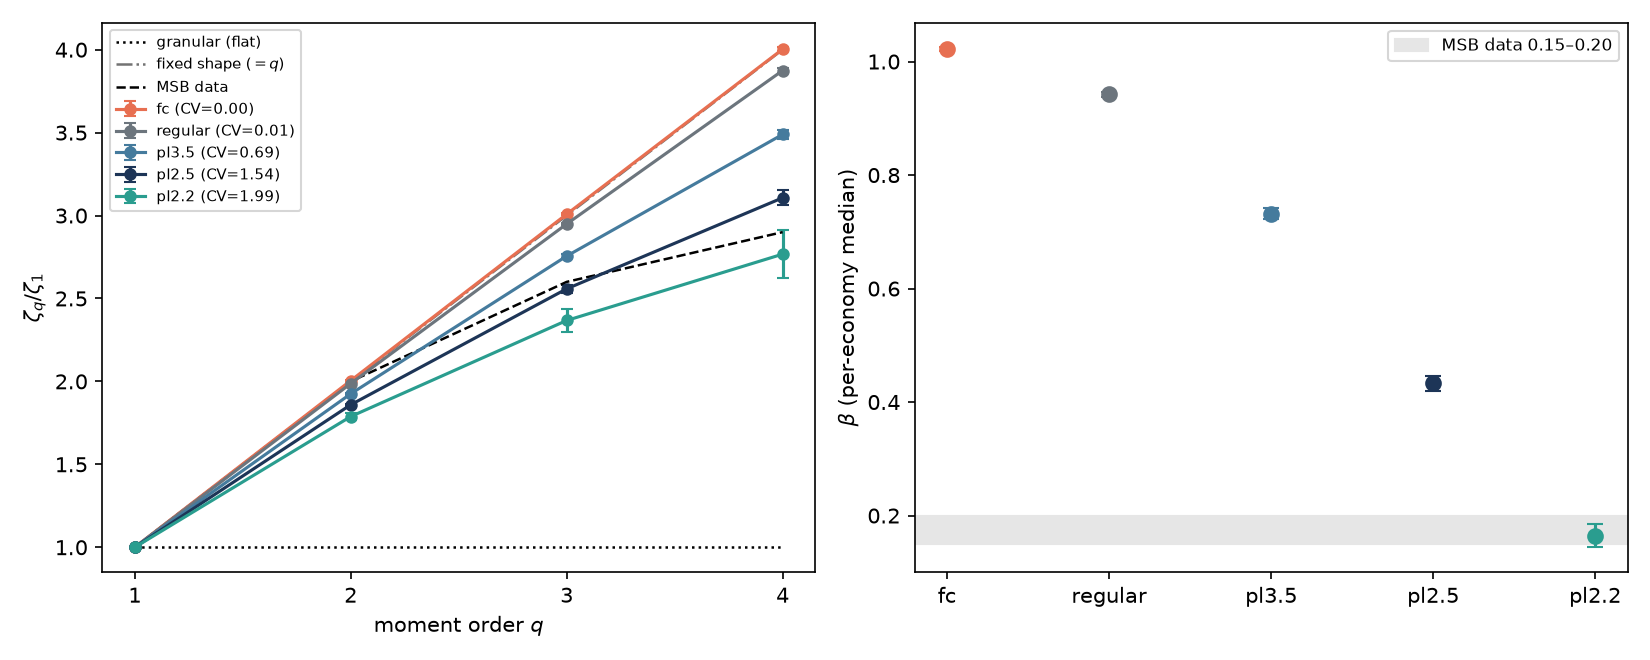
\includegraphics[width=\linewidth]{meandeg_topology.png}
    \caption{The graph generates the size-conditioned statistics. Five degree
    distributions at the same operating point, mean degree and disorder, twenty economies
    each ($N = 8000$; the ordering is unchanged at $N = 16000$). \panel{Left}: quenched
    multiscaling ratios. The homogeneous graphs (fully connected, regular) sit on the
    fixed-shape line $\zeta_q/\zeta_1 = q$ (no multiscaling) and the curve bends
    toward the data as the degree distribution broadens (CV is the coefficient of
    variation of the degrees); only the infinite-variance power-law graphs reach the
    neighbourhood of the empirical curve. \panel{Right}: the size--variance exponent falls from $\beta \approx 1$
    on homogeneous graphs toward the empirical range as heterogeneity grows.
    Table~\ref{tab:growing-topology} gives the numbers.}
    \label{fig:growing-topology}
\end{figure}

\begin{table}[htbp]
    \centering
    \begin{tabular}{lcccccc}
        \hline
        graph & survive & $\beta$ & $\zeta_2/\zeta_1$ & $\zeta_3/\zeta_1$
              & $\zeta_4/\zeta_1$ & tent exkurt \\
        \hline
        fully connected & $20/20$ & $1.02$ & $2.00$ & $3.01$ & $4.00$ & $11$ \\
        regular         & $20/20$ & $0.94$ & $1.99$ & $2.95$ & $3.87$ & $11$ \\
        power law $3.5$ & $20/20$ & $0.73$ & $1.93$ & $2.76$ & $3.49$ & $8$  \\
        power law $2.5$ & $20/20$ & $0.43$ & $1.86$ & $2.56$ & $3.11$ & $8$  \\
        power law $2.2$ & $20/20$ & $0.17$ & $1.79$ & $2.37$ & $2.77$ & $9$  \\
        \hline
        fixed shape     &         &        & $2$    & $3$    & $4$    &      \\
        MSB data        &         & $0.15$--$0.20$ & $2.0$ & $2.6$ & $2.9$ &  \\
        \hline
    \end{tabular}
    \caption{The topology sweep of Figure~\ref{fig:growing-topology} in numbers: the same
    operating point, disorder and mean degree, only the degree distribution swapped
    ($N = 8000$, twenty realizations per graph). $\beta$ is the median per-economy
    decline-branch slope (standard errors $0.003$--$0.020$); the ratios are quenched means
    over economies (standard errors $\le 0.05$, the power-law-$2.2$ ratios up to
    $0.14$); the tent excess kurtosis
    is the per-economy median. Homogeneous graphs sit on the fixed-shape row to within
    error, the power-law-$2.5$ graph approaches the empirical ratio row, and the
    power-law-$2.2$ graph places $\beta$ inside the empirical band at this size with
    ratios slightly below the data; the growth
    tent stays fat on every topology. (An exponential-degree graph at the same operating
    point sits at the edge of the freezing transition, losing a third of its realizations,
    and is omitted.)}
    \label{tab:growing-topology}
\end{table}

This ablation is the counterpart of a second one, on the disorder itself.
Table~\ref{tab:growing-ablation} sweeps $\sigma$ at fixed $\mu$, $\lambda$
and $N$. Below the threshold $\sigma_c$ the dynamics freeze: the late-time
growth fluctuations are zero to the precision quoted, the shape has relaxed to a fixed
point, and there is no fluctuating state to measure. The persistent fluctuations and
the fat-tailed tent appear only once $\sigma$ crosses $\sigma_c$, growing with the
disorder. With no noise in the model, the fluctuations can come only from the disorder,
and removing it removes them entirely. The two ablations together assign the phenomena
to their sources: the disorder makes the economy fluctuate and gives the growth
distribution its heavy tails; the degree heterogeneity of the graph turns those
fluctuations into the size-conditioned structure (the low exponent and the
multiscaling) that the data show.

\begin{table}[h]
    \centering
    \begin{tabular}{rccc}
        \hline
        $\sigma$ & growth fluctuation & excess kurtosis & fat-tailed tent? \\
        \hline
        $0.00$ & $0.000$ & --   & no  \\
        $0.50$ & $0.000$ & --   & no  \\
        $1.00$ & $0.000$ & --   & no  \\
        $1.41$ & $0.000$ & --   & no  \\
        $1.60$ & $0.085$ & $14$ & yes \\
        $1.75$ & $0.175$ & $14$ & yes \\
        \hline
    \end{tabular}
    \caption{Disorder ablation at $\mu = -1.76$, $\lambda = 10^{-3}$, $N = 3200$ on a
    power-law graph. ``Growth fluctuation'' is the standard deviation of the pooled
    late-window growth rates. Below the chaotic threshold $\sigma_c$ the state
    freezes (growth fluctuation zero to the precision quoted) and there is no genuine
    fluctuating distribution to characterize, so the kurtosis is left blank; the
    persistent fluctuations and the fat-tailed tent switch on only once $\sigma$ crosses
    $\sigma_c$. (A nonzero $\beta$ can still be fitted below threshold. It reflects a frozen
    state during its relaxation, the V transient of the absolute critical model, and says
    nothing about a stationary fluctuating law.)}
    \label{tab:growing-ablation}
\end{table}

The interactions-only origin also separates this model from the simplest alternatives. A
mean-field multiplicative model with injected noise already gives a growing economy with a
stationary heavy-tailed size distribution \citep{bouchaudmezard2000}, but there the
fluctuations are external and there is no network. Here the same growing aggregate, the heavy tails,
and the slow size--variance decay arise together from the disordered
interactions, and the size-conditioned structure from the topology that carries them.

\section{From degree to size: survival under competition}
\label{sec:growing-degree-size}

The degree-dependent field variance that carries the graph into the statistics also
acts on the individual firm, and its effect has two parts: degree sets size but barely
touches volatility, and it sets size not by advantaging the connected firm but by
widening the spread of outcomes among connected firms, most of which lose.

The first part is the observation itself, shown in Fig.~\ref{fig:growing-degree-size}.
Measured per economy at the operating point, a firm's mean size rises with its degree, Spearman
correlation $+0.41$ (range $+0.37$ to $+0.44$ across ten economies of $N = 16000$),
positive in every realization, and the relation is a power law,
$\bar S \sim k^{\delta}$ with $\delta = 0.56 \pm 0.02$. Unlike the size--variance
exponent, $\delta$ is converged at our sizes: it is $0.57 \pm 0.03$ at $N = 8000$ and
unchanged at $N = 16000$. The firm's volatility, by contrast, is nearly flat in its
degree (Spearman $+0.16$, right panel), and the flatness is a near-cancellation of two
opposing dependences. Fitted jointly across the firms of twelve economies at
$N = 8000$, the volatility scales as $\sigma_i \propto k_i^{\,b}\,\bar S_i^{-a}$ with
$b = 0.486 \pm 0.012$ and $a = 0.588 \pm 0.015$: at fixed size a hub is noisier, the
$k_i/C$ field variance of Section~\ref{sec:growing-graph} surfacing directly, but the
size that noise procures quiets the firm through the size--variance law, and the two
compose to $\sigma \propto k^{\,b - a\delta} \approx k^{+0.16}$ with $\delta = 0.56$,
the weak residual the figure shows. Degree acts on size, and the
volatility inherits only what the size--variance law leaves over.

\begin{figure}[htbp]
    \centering
    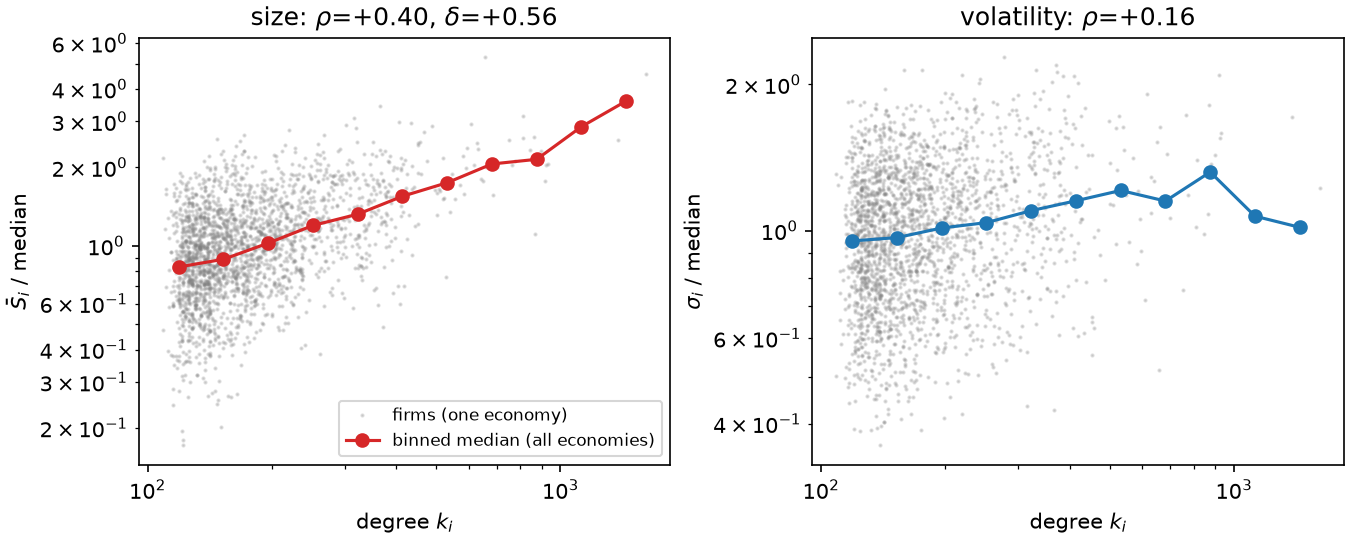
\includegraphics[width=\linewidth]{meandeg_degree_size.png}
    \caption{Degree and the individual firm, ten economies of $N = 16000$ ($C = 400$),
    each economy's sizes and volatilities normalized by its own median. \panel{Left}:
    mean size against degree; the binned median (across all economies) rises as a power
    law $\bar S \sim k^{\delta}$, $\delta = 0.56 \pm 0.02$, per-economy Spearman
    correlation $+0.41$. \panel{Right}: volatility against degree is nearly flat
    (Spearman $+0.16$): the two opposing degree dependences, the noise rising with
    degree and the size it procures quieting the firm, nearly cancel, and
    $\sigma \sim k^{+0.16}$ is the residual.}
    \label{fig:growing-degree-size}
\end{figure}

The second part is the selection behind the relation. Under competition ($\mu < 0$) a
hub has more competitors and feels a mean suppression that grows with its connectivity,
and most hubs indeed lose: the survival probability falls monotonically with degree,
from $0.22 \pm 0.05$ in the lowest degree bin to $0.02 \pm 0.02$ in the highest. A
firm's couplings are also a quenched draw whose spread widens with degree, and
conditioning on survival reverses the correlation between the average interaction field
a firm sits in and its degree, from $-0.27$ over all firms to $+0.35$ among the
survivors, so the hubs that remain are those whose draw came out favourable, and their
sizes track those favourable fields. The field the survivors are drawn from is
fat-tailed, a sum over neighbours weighted by their heavy-tailed sizes, and the largest
survivors live in exactly that tail.

A final control assigns the diversity itself to the competition. Setting $\mu = 0$ at
the same disorder removes the mean suppression, and with it the coexistence: the
economy condenses onto a handful of firms (survival below $0.2\%$ in every
realization), so the same penalty that eliminates the typical hub holds the rest of the
economy in coexistence. Connectivity widens the quenched draw a firm receives,
competition removes most of the widened draws, and the surviving tail is large in
proportion to the widening. As in Section~\ref{sec:growing-graph}, the firm-to-firm
structure is quenched, frozen into the realized couplings, and the dynamics select and
expose it.
